Structure:
\begin{itemize}
    \item[State of things]
    \item two large trends \means distribution + heterogeneity vs need for security+safety+verification 
    \item this starts at the OS level, i.e. distribute processes among cpus, compute on cpu/gpu/special purpose HW (e.g. signal processing in mobiles)
    \item[Problem with that]
    \item On the one hand, distribution facilitates isolation \means good
    \item On the other hand, distribution comes with concurrency and increased complexity of programming (incl. new layer of abstraction) and they are the "natural enemy" of verification
    \item another issue, in particular when systems need to be secure is the adaptation overhead to new execution scenarios
    \item[Approache so far]
    \item we can see the struggle is real 
    \item cite approaches to verfiy OSes
    \item cite e.g. Model Checking for Distributed Sytems 
    \item[Our approach]
    \item verify the sequential, local code \means have verified transformations applied \means get a verified distributed program
    \item classical sceanrio on OS level is a NW stack. It connects user App to the outside wordl, uses different system services and in particular (nw) device drivers which is relevant because device drivers are notorious for bugs
    \item \emph{what does ohua do so far}
    \item \emph{what did we do with smoltcp and why is interesting}
    \item \emph{what did we show}
\end{itemize}

\todo[inline]{Can I get e reference to Compositionality papers .. It woudl be awesome if we could get the link to \means "we transform a verified object into a verified category, i.e. composable, verified objects"}

Actual Problem description
\begin{itemize}
    \item what we have is a library called smoltcp, that implements the network stack in userspace \means it can be used in a unikernel setting, where such system services are not part of the kernel
    \item what we want is the ability to compile applications build with smoltcp to run in a microkernel setting in particular in the M$^3$ hw-os system
    \item Why is this interesting:
    \begin{enumerate}
        \item Transformation to message passing: In it's current state, smoltcp actually combines the TCP/IP stack and an interface to the actual physical layer. The according parts of the library are coupled via shared references and invoke each other via normal function calls. This works well in unikernels, as well as in monoliths (implemented in user space vs. kernel space respectively). In a microkernel, we might want to separate this two functionalities to use and scale them independently. This requires components to interact not vie function calls and shared references but via IPC. SO one aspect of the problem is to investigate which constraints the isolation of components imposes on the code and which transformations achieve a compatible structure. Exmpl: We can not call functions with mutable references any more because the sematics of such calls change, when components are separated and objects are serialized upon invocation.
        \item Local State: Smoltcp is a good example for an application with interacting states. From a bird's eye view we can basically distinguish three states, the server application holding e.g. requests currently to process, the network stack holding for example socket states and the network interface abstraction \todo[inline]{I don't think thats a stateful thing, it's basically a source/sink abstraction to the system}. 
        
        \todo[inline]{describe a) the state locality problem i.e. write the code such that no internal function will try to access another components state outside the 'flow' b) rewrite it such a way, that Ohua identifies the components we want}
        Take the example in  ... 
        So the question is, can we a) identify all syntactic constructs that lead to states being transferred in the resulting DFG and b) identify code transformations to avoid this (on the level of input code)
        \item Compile from Uni- to Microkernel \question{$M^3$ already is a Microkernel using smoltcp as a userspace service, so how to describe exactly what's the point here?}
        \item True, but we do not target OS1 \means OS2 but only OS1 mono/unikernel \means OS1 microkernel \textcolor{gray}{Transpile to another Operating System: Current Ohua integrations \todo[inline]{Check if this hold historically} produced concurrent version of a sequential input program both running on in basically the same runtime environment i.e. the OS interface and standard components of the language (e.g. the Rust standard library). This is not the case for M3. M3 does (to the date this work is written) not support the Rust standard library. }
        \todo[inline]{As it supports libc, and smoltcp doesn't need std this could be no big thing for now. However it is a general problem to consider, also with respect to cloud environments, that (out-of-scope) parts of the compiled software use functions, that rely on system interfaces being present or having a particular semantic, e.g. opening files, writing to stdout/err, trying to access sytem services as time or randomness}
        \item Extending the Rust subset of Ohua: Ohua is currently lacking some general as well as Rust specific language constructs. Most importantly compiling a condition guarded loop (\code{while} or \code{do-while}) is currently not supported. Further Ohua does currently not accept structs, impl functions and trait implementations in the compile scope (i.e. they can be used only in the called libraries). So another goal is to describe and implement code transformations (or, if necessary, remaining restrictions) to accept struct and impl definitions. 
        
        \item Exemplify Usage: The last point is to demonstrate the domain knowledge required from the programmer. Ohua obviously can not tell, for any two structs or modules of smoltcp and applications using it, if they should end up in the same service or not. The level and lines of separation have to be provided by the programmer. Specifically the composition of function calls in the compilation scope determines the structure of the derived DFG. \todo[inline]{example}
    \end{enumerate}
   
\end{itemize}
    \begin{figure}[H]
    \centering
    
    \begin{subfigure}[b]{0.6\textwidth}
         \centering
         \begin{minted}{rust}
   fn somefun() -> i32 {
       let mut mStruct = MS::default();
       let i = mStruct.f();
       let j = mStruct.g();
       calculate(i,j)
   }       
            \end{minted}
         \caption{Multiple calls to a struct}
         \label{multCalls}
     \end{subfigure}
     %\hfill
     \par\bigskip
     \begin{subfigure}[b]{0.6\textwidth}
         \centering
         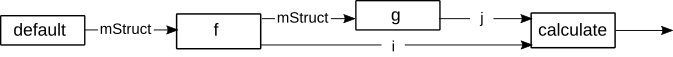
\includegraphics[width=\textwidth]{figures/graph_state_moved.png}
         \caption{Resulting data flow graph}
         \label{DFGStateMoved}
     \end{subfigure}
    \par\bigskip
     \begin{subfigure}[b]{0.6\textwidth}
         \centering
         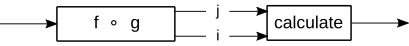
\includegraphics[width=0.6\textwidth]{figures/graph_state_not_moved.png}
         \caption{Target data flow graph}
         \label{DFGStateNotMoved}
     \end{subfigure}
    \caption{}
    \label{fig:SimpleStateUseFigure}
    \end{figure}
    
    \todo[inline]{Explain the contingency from SharedMemory programming model, over M3 to Cloud deployment: maybe Mention in Intro, details in the background}
    Describe essential differences at: 
    \begin{itemize}
        \item Is it one program or do we compile/deploy different programs?  $\rightarrow$ are types known/inferable at compile time/do they have to be? $\rightarrow$ Do we compile for the same OS? \\
         $\Rightarrow$ points above have consequences e.g. 
        \item What are the constraints on types being passed (serializable, are \rust{dyn} allowed, are generics allowed, who takes care of compatibility in case of different OSs)? 
        \item What are other constraints for the programmer (e.g. using system specific interfaces for components) How much packaging does the Compiler have to do (e.g. assorting libraries to components)? 
        \item (How) do we need to handle errors/panics?(in a 'one program' scenario it's one panic to crash them all. How is it in M3? It's even more complex in 'really' distributed scenarios as there are different reasons components might not answer and even if they answer with an error we might have different strategies to handle.)
        \item Do we need to build in a shut down mechanism? 
        \item Can/Should the Compiler be able to detect system interaction and tailor them?        
    \end{itemize}
    
    
    \todo[inline]{Important Point I don't know where to put yet and also needs elaboration:}
    \note{The transformation we will extract from the rewriting process are to some degree actually extensions of Ohua programming model. The model currently already enforces 1) variables to be either used as state, or as variable i.e.\means no sending of states and 2) states from outside the loop scope to be only used once inside loop or recursion \means linearity inside loops. What is not enforced currently is, that states in general are used only once, i.e. outside loops or when created inside loops states can be used more than once \means so no linearity here.}

    
\todo[inline]{Example Rust 4 Unikernel \cite{Rust4Unikernel}}
\todo[inline]{Formal Verification eg for L4 derivatives as motivation \cite{sL4Verf}}
